%\documentclass[10pt,a4paper,twocolumn]{article}
%\documentclass[10pt,a4paper]{article}

% Extra packages
%\usepackage{fullpage}
%\usepackage[utf8]{inputenc}
%\usepackage{amsmath}
%\usepackage{amsfonts}
%\usepackage{amssymb}
%\usepackage{graphicx}
%\usepackage{hyperref}

%\usepackage{graphicx}
%\usepackage{caption}
%\usepackage{subcaption}

% Document description
\title{Convergence of modified interpolation kernel for treating diffusion}
\author{Lento Manickathan, 1544101.\\Aerodynamics and Wind energy}

% Begin of main body
%\begin{document}

% Show title
%\maketitle

% Main content

\section{Introduction to modified interpolation kernel for treating diffusion}
The diffusion method that is applied here has been proposed by Shankar and Van Dommelen \cite{Shankar1996} and the modified ${{{\rm{M'}}}_4}$ interpolation kernel has been derived by Ghoniem and Wee \cite{Wee2006} and was also applied by Speck \cite{Speck2011}. The diffusion is simulated by the modified interpolation kernel during the remeshing process. During remeshing, the heat equation is satisfied by transferring the correct fraction of circulation to produce the proper amount of diffusion. The ${{{\rm{M'}}}_4}$ kernel was modified to treat the diffusion and is given by: 

\begin{equation}
{{{\rm{M'}}}_4}\left( {\xi ,c} \right) =
  \begin{cases}
   {1 - \frac{{5{\xi ^2}}}{2} + \frac{{3{{\left| \xi  \right|}^3}}}{2} - {c^2}\left( {2 - 9{\xi ^2} + 6{{\left| \xi  \right|}^3}} \right)} & {\left| \xi \right|} < 1, \\
   \frac{1}{2}{\left( {2 - \left| \xi  \right|} \right)^2}\left( {1 - \left| \xi  \right|} \right) - {c^2}{\left( {2 - \left| \xi  \right|} \right)^2}\left( {1 - 2\left| \xi  \right|} \right) & 1 \le {\left| \xi \right|} < 2,\\
   0 & 2 \le \left| \xi \right|,
  \end{cases}
\label{eq:modInterpKernel}
\end{equation}

where 

\begin{equation}
c = \frac{\sqrt{\nu \Delta t_d}}{\Delta x},
\label{eq:c2}
\end{equation}

and corresponds to the transfer quantity for diffusion. The $\nu$ denotes the viscosity of the fluid, $t_d$ is the diffusion time step and $\Delta x$ is the blob spacing. When $c \rightarrow 0$, the interpolation kernel turns to the classical non-diffusion kernel.  This modified interpolation kernel conserves the circulation of each vortex and also satisfies the conservation of linear and angular momentum of the vorticies.\\

The vortex method employs the viscous splitting procedure, where the vortex blobs are convected first and is then diffused through the remeshing process using the modified interpolation kernel. The advantage of this methodology is that the convection process is not constrained by the CFL condition. So, the convection time step size can be different than from the diffusion time step size and the diffusion time step size is a multiple of the convection time step size depending on the redistribution frequency $f_{redist}$. Therefore, the constrained that is imposed on the redistribution frequency is the stability bounds of the modified interpolation kernel. Analyzing the amplification factor and the phase error of the modified interpolation kernel in the Fourier space requires that the $c^2$ should be as follows:


\begin{equation}
\frac{1}{6} \le c^2 \le \frac{1}{2}.
\label{eq:c2stability}
\end{equation}

This will ensure the stability of the problem and will suppress any spurious oscillations and ensure that it is a non-negative interpolation kernel with non-negative redistribution fractions.

\section{Errors in Blob Initialization}
To verify the accuracy of the diffusion process, the error of the discrete solution was compared against the analytical solution of the Lamb-Oseen vortex where the vorticity field

\begin{equation}
\omega\left(x,t\right) = \frac{\Gamma_o}{4\pi \nu t} \exp \left(-\frac{r^2}{4 \nu t} \right),
\label{eq:LambOseen}
\end{equation}

was used as the analytical solution for a given viscosity $\nu$ at a given time $t$ with a unit circulation $\Gamma_o$. In order to quantify the error generated during discretization, the discrete $L^2$-norm error was calculated as 

\begin{equation}
{\left\| {{\omega ^{{\rm{exact}}}} - {\omega ^{{\rm{discrete}}}}} \right\|_2} = {\left( {\sum\limits_i {{{\left| {{\omega ^{{\rm{exact}}}}({{\bf{x}}_i}) - {\omega ^{{\rm{discrete}}}}({{\bf{x}}_i})} \right|}^2}\Delta x\Delta y} } \right)^{\frac{1}{2}}},
\label{eq:L2normEq}
\end{equation} 	

and the discrete maximum relative error in vorticity was evaluated as follows:

\begin{equation}
{\left\| {{\omega ^{{\rm{exact}}}} - {\omega ^{{\rm{discrete}}}}} \right\|_\infty } = \frac{{\max \left\{ {\left| {{\omega ^{{\rm{exact}}}}({{\bf{x}}_i}) - {\omega ^{{\rm{discrete}}}}({{\bf{x}}_i})} \right|:i \in {\mathcal{S}}} \right\}}}{{\max \left\{ {\left| {{\omega ^{{\rm{exact}}}}({{\bf{x}}_i})} \right|:i \in {\mathcal{S}}} \right\}}}.
\label{eq:maxRelEq}
\end{equation}

During the initial discretization, it was seen that in order to obtain the correct vorticity field, you need to take in account of the numerical diffusion. As Barba had shown in \cite{Barba2004a}, in order to properly account for the diffusion effect when discretization with gaussian blobs (with $k=2$), a time-shift correction equivalent to shifting the initial time by $\sigma^2/2\nu$ needs to be applied. This follows directly from the discretization of the general solution of the heat equation with these gaussian cores. With this proper time-shifting, you can ensure the accurate initialization of the Lamb-Oseen vortex for the error evaluations. \\

An alternate method of taking account for the gaussian approximation is the Beale's iterative method for circulation processing. The concept is based on iteratively improving the circulation values of the gaussian blobs so that it gives a better approximation of the local vorticity that the blobs are trying to represent. The downside to this processing is that the influence matrix for the calculation is $\mathcal{O}(N^2)$ and requires large computational resources.

\section{Importance of initial conditions}



\begin{itemize}
\item Comparing $\nu=0.01$ and $\nu=0.0005$ with various starting times. Show the growth in error. 
\item Compare various correction methods for initial discretization. Beale vs. time-shifting
\end{itemize}

\section{Convergence of the vortex method with diffusion}
The discretization errors of the vortex method was evaluated to check for the convergence of its error to the exact solution. If the modified interpolation kernel was accurately implemented into the vortex method, the spatial and the temporal discretization error of the vortex method should converge as you refine the parameters. When checking for discretization error a given parameter, all the other parameters was kept constant and at a very high resolution. This ensured that the significant error emerges from the discretization of the chosen parameter. For the initial investigations, this meant that the $c^2$ parameter of the kernel diffusion term was also varying dependent on the discretization parameter. This could indirect influence on the convergence rate, as diffusion term was varying for each discrete value. So, a second investigation was done, where the $c^2$ parameters was kept constant by varying the appropriate values.

To ensure that other numerical error does not dominate and the consistency of the simulations, all the variables were carefully chosen and are tabulated in table \ref{tab:refinementParameters}.\\

\begin{table}[hbt]
\centering
	\begin{tabular}{|l|r|}
	\hline \textbf{Parameters} 					& \textbf{Value} \\
	\hline Domain $\Omega$ 						& $[-2, 2]^2$ \\
	Overlap ratio $\Delta h/\sigma$  	& 0.5  \\ 
	Viscous time scale $\tau$ 			& 0.0200 to 0.0250 \\
	Time step scheme 					& RK4 \\
	Vortex viscosity $\nu$ 				& [0.01, 0.0005] \\
	Vortex Circulation Strength $\Gamma$ & $2 \pi$ \\
	Vortex Reynolds Number Re 			& [50, 2000] \\
	Vortex Reynolds Number Re 			& [50, 2000] \\
	Kernel diffusion parameter $c^2$		& $1/6$, $1/4$, $1/2$ \\
	Redistribution frequency $f_{redist}$& 1 \\
	Population control $\Gamma_{min}$ 	& \texttt{eps} $ = 2.2e$\textrm{-}$16$\\
	Population control frequency $f_{pc}$& 1 \\
	\hline 
	\end{tabular} 
\caption{Refinement study parameters}
\label{tab:refinementParameters}
\end{table}


\subsection{Blob density refinement study}
In order to investigate the convergence of the error and as the spatial discretization is refined, a blob density refinement study was undertaken. By increasing the number of blob cores to represent the given vortex, the discrete approximation of the vortex should converge to the exact solution. In order words, as the spatial discretization $\Delta y$ and $\Delta y$ is reduced, the error should converge.

During the investigation of the blob density (number of particles) refinement, the time step was maintained at a minimum to reduce its error, $\delta T = 0.05$. Investigation was done for two viscous cases, as shown in table \ref{tab:refinementParameters}. This results in time step parameters as shown in table \ref{tab:spatialRefinementParameters}.

\begin{table}[hbt]
\centering
	\begin{tabular}{|l|r|r|}
	\hline \textbf{Parameters} 	& \textbf{$\nu = 0.01$} & \textbf{$\nu = 0.0005$}\\
	\hline Start time $\tau/\nu$    & 2 & 40 \\				
	Stop time  $\tau/\nu$ 	& 2.5 & 50 \\
	Number of steps 			& 10 & 200 \\
	Number of blobs 			& [73, 86, 98, 108, 118, 126] & [327, 386, 438, 484, 527, 566]\\
	\hline
	\end{tabular}
\caption{Blob density refinement study parameters}
\label{tab:spatialRefinementParameters}	
\end{table}

The results of the spatial refinement is shown in figure \ref{fig:wErrorVSdx_varyingC2}. 

\begin{figure}[!tbhp]
\centering
	\begin{subfigure}{0.48\textwidth}
		\centering
		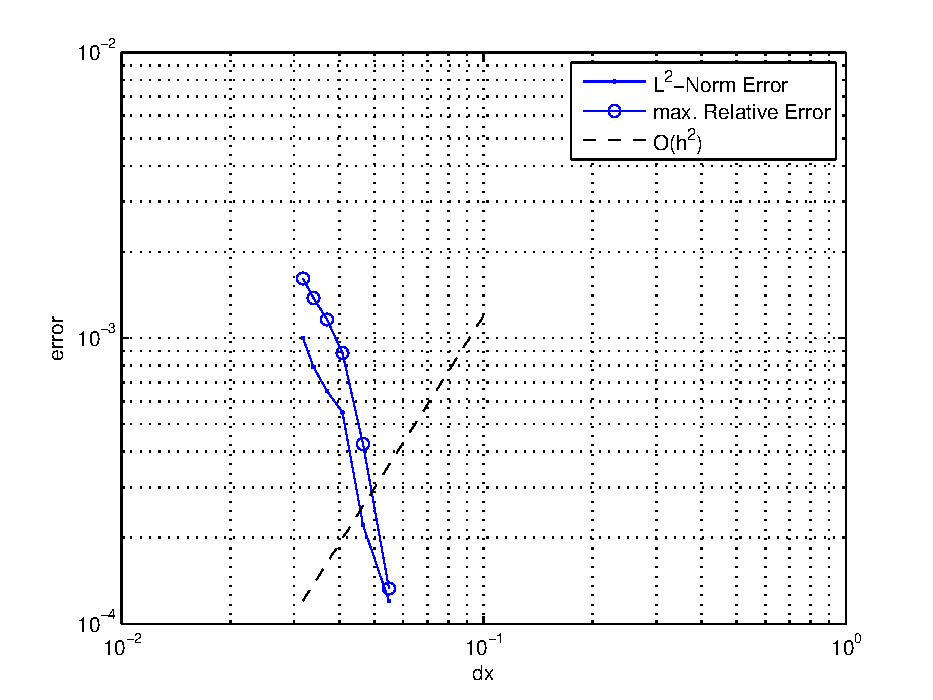
\includegraphics[width=\textwidth]{./figures/wErrorVSdx_nu001_c2vary.pdf}	
		\caption{$\nu=0.01$}
	\end{subfigure}
	\begin{subfigure}{0.48\textwidth}
		\centering
		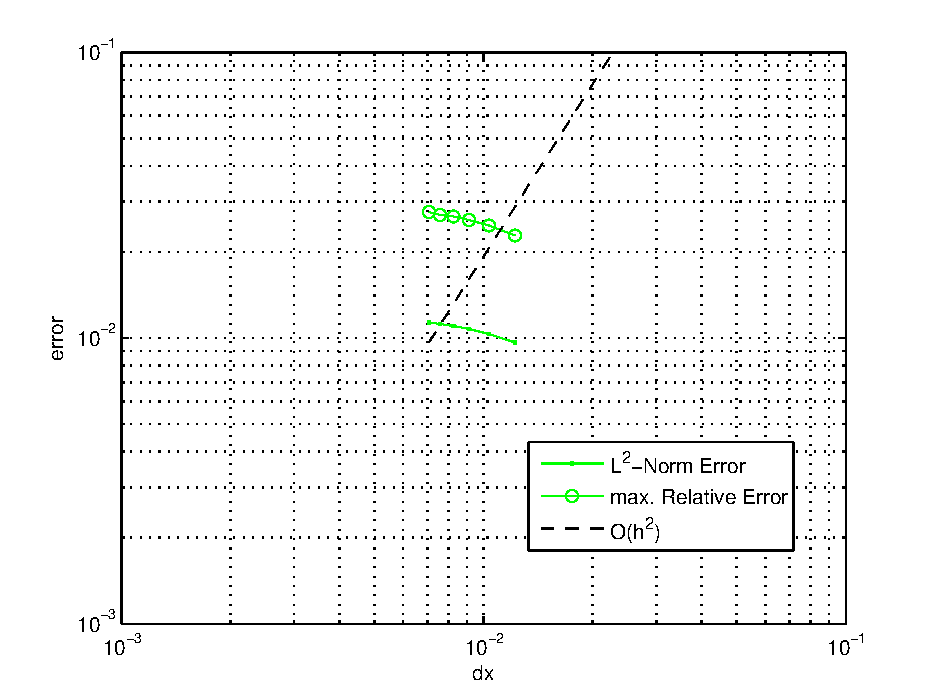
\includegraphics[width=\textwidth]{./figures/wErrorVSdx_nu00005_c2vary.pdf}	
		\caption{$\nu=0.0005$}
	\end{subfigure}
\caption{Spatial refinement with a varying $c^2$}
\label{fig:wErrorVSdx_varyingC2}
\end{figure}

It is evident that the order of convergence does not match the predicted one. This is because of the one key parameter, the kernel diffusion parameter $c^2$. We assume that as the number of particles (i.e blob density) increases, the spatial discretization $\Delta h$ reduces thereby resolving the Lamb-Oseen vortex to greater detail. However, from equation \ref{eq:c2} we see that if viscosity $nu$ and time step $\Delta T$ is constant then $\Delta $ is inverse proportional to kernel diffusion parameter $c^2$. This means that the $c^2$ parameter is increasing and has a direct influence of the damping of the numerical oscillations. Therefore, as the $c^2$ increase, the growth in error might be more dominant and could have an effect on the spatial refinement study.\\

So, to have a proper comparison, the spatial refinement study was done with keeping the $c^2$ parameter constant, figure \ref{fig:wErrorVSdx_constantC2}.

\begin{figure}[!tbhp]
\centering
	\begin{subfigure}{0.48\textwidth}
		\centering
		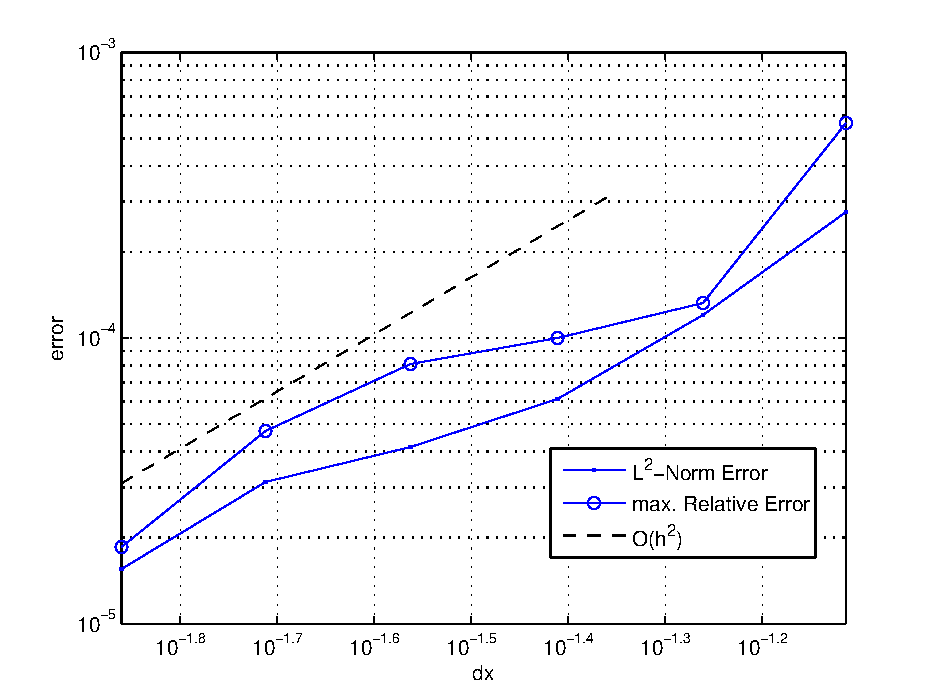
\includegraphics[width=\textwidth]{./figures/wErrorVSdx_nu0p01_constantc2.pdf}	
		\caption{$\nu=0.01$}
	\end{subfigure}
	\begin{subfigure}{0.48\textwidth}
		\centering
		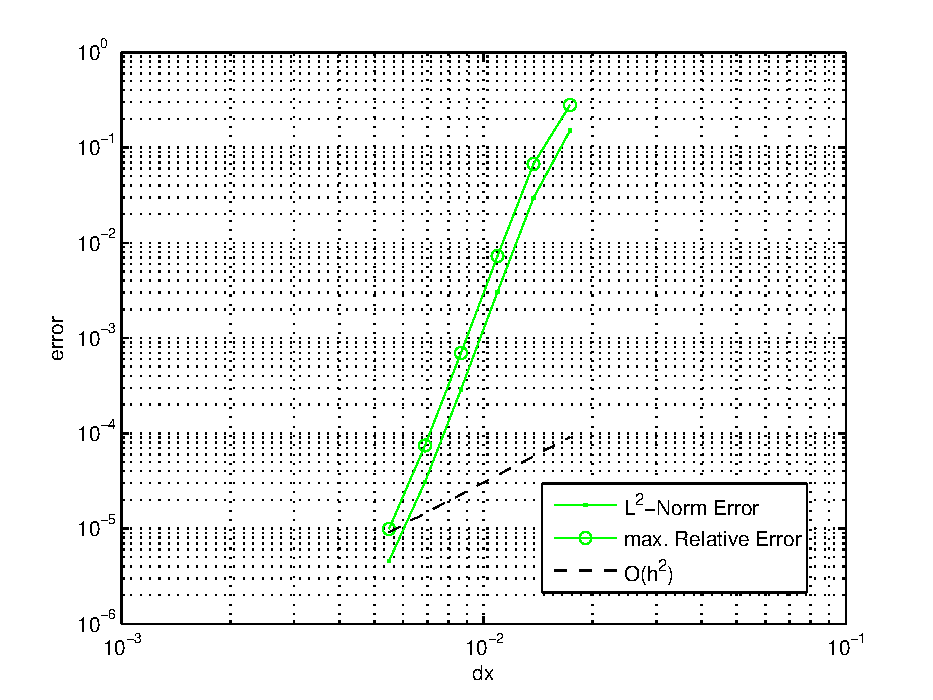
\includegraphics[width=\textwidth]{./figures/wErrorVSdx_nu0p0005_constantc2.pdf}	
		\caption{$\nu=0.0005$}
	\end{subfigure}
\caption{Spatial refinement with a constant $c^2=1/6$}
\label{fig:wErrorVSdx_constantC2}
\end{figure}

Now we can see that the error converges as you reduced the blob mesh size. This is the correct trend that we are looking for.

\subsection{Spatial refinement for various kernel diffusion parameter}

\begin{figure}[!tbhp]
\centering
	\begin{subfigure}{0.48\textwidth}
		\centering
		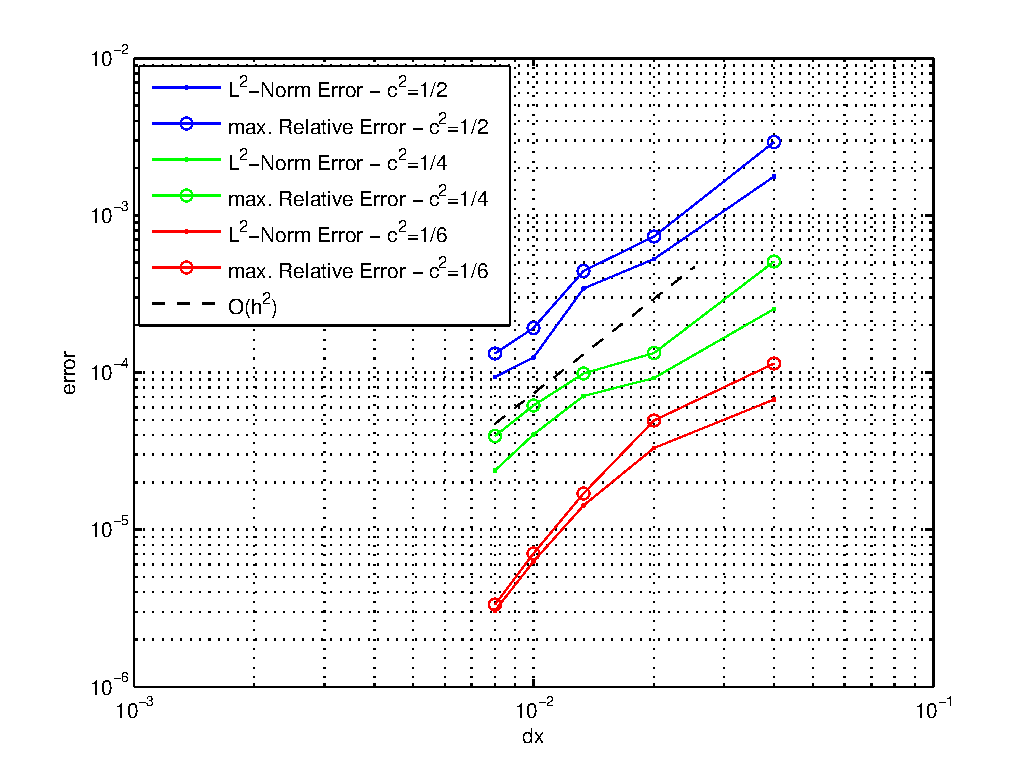
\includegraphics[width=\textwidth]{./figures/wErrorVSdx_nu0p01_variousC2.pdf}	
		\caption{$\nu=0.01$}
	\end{subfigure}
	\begin{subfigure}{0.48\textwidth}
		\centering
		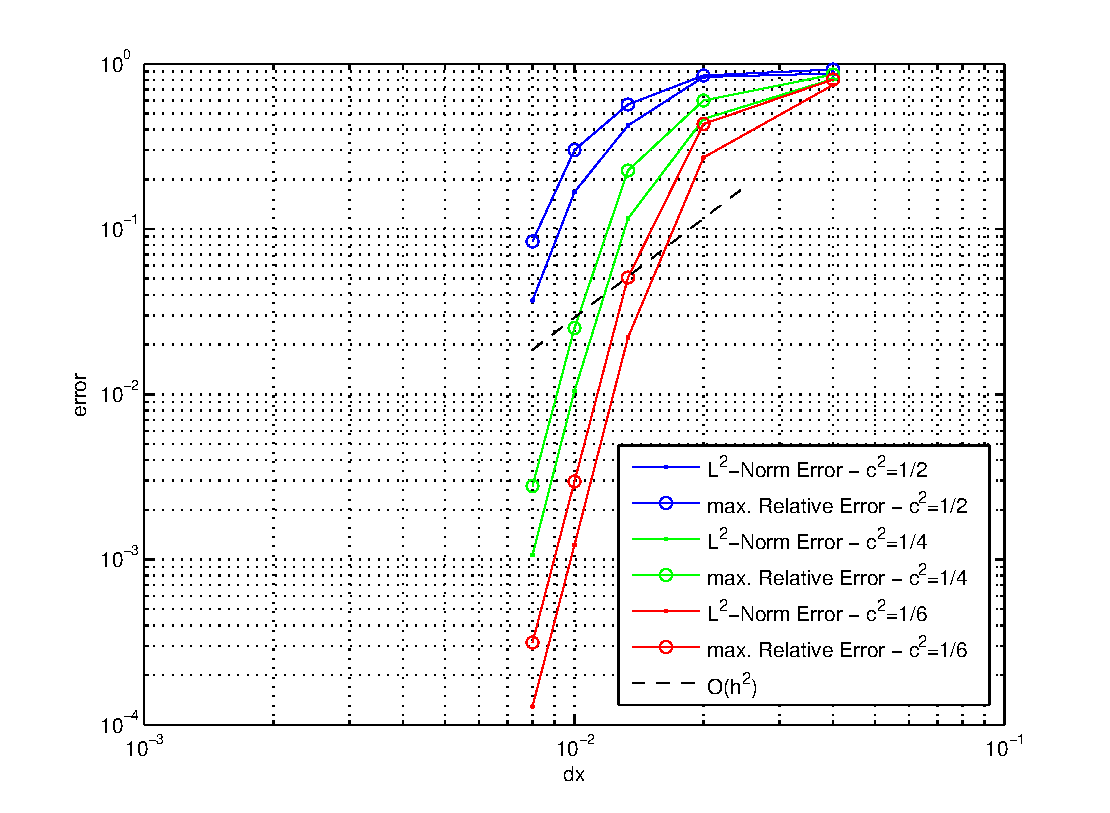
\includegraphics[width=\textwidth]{./figures/wErrorVSdx_nu0p0005_variousC2.pdf}	
		\caption{$\nu=0.0005$}
	\end{subfigure}
\caption{Spatial refinment for various $c^2$ parameters, $c^2 = [\frac{1}{6}, \frac{1}{4}, \frac{1}{2}]$}
\label{fig:wErrorVSdx_variousC2}
\end{figure}



\subsection{Time Step refinement study}

\begin{figure}[!tbhp]
\centering
	\begin{subfigure}{0.48\textwidth}
		\centering
		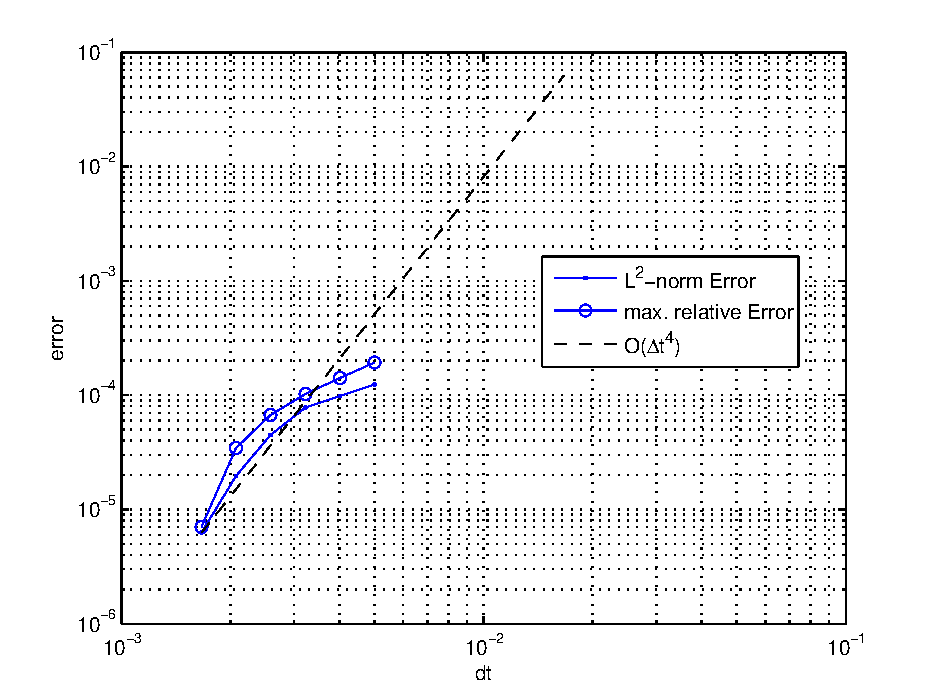
\includegraphics[width=\textwidth]{./figures/wErrorVSdt_nu0p01_varyingC2.pdf}	
		\caption{$\nu=0.01$}
	\end{subfigure}
	\begin{subfigure}{0.48\textwidth}
		\centering
		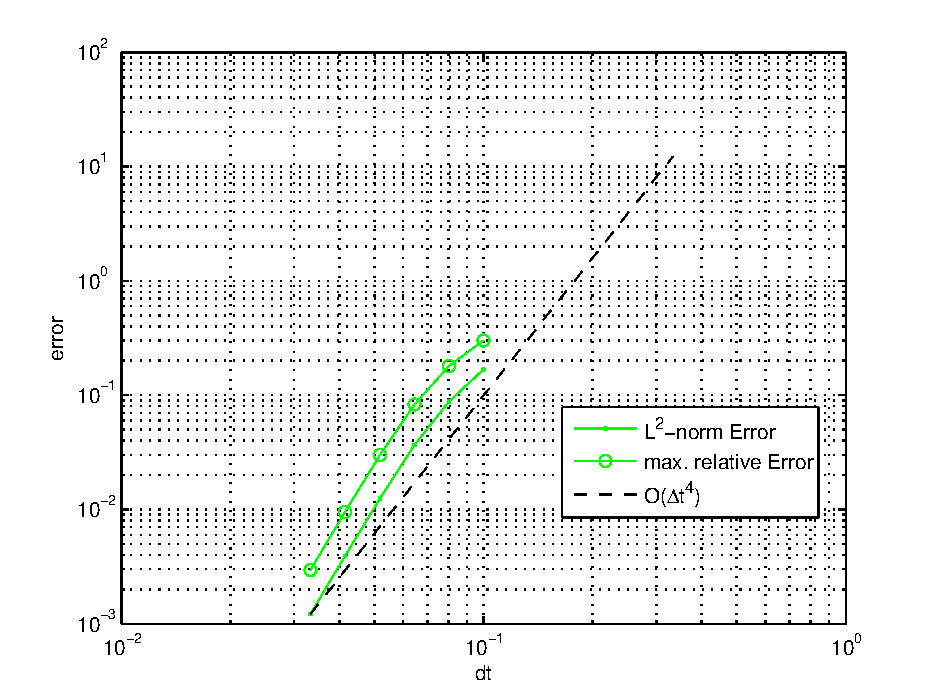
\includegraphics[width=\textwidth]{./figures/wErrorVSdt_nu0p0005_varyingC2.pdf}	
		\caption{$\nu=0.0005$}
	\end{subfigure}
\caption{Time Step refinement with a varying $c^2$}
\label{fig:wErrorVSdt_varyingC2}
\end{figure}





% End of main body
\newpage

% Bibliography
%\bibliographystyle{plain}
%\bibliography{../../Literature/library}

% End of document
%\end{document}